\section{Interface} % (fold)
\label{sub:interface}
  A interface de usuário é onde ocorre a interação entre humanos e máquinas, o objetivo desta interação é a operação e controle efetivos da máquina pelo usuário e o feedback desta, que auxilia o operador na tomada de decisões operacionais.

  Tendo em vista isso o aspirador terá uma plataforma web que contará com uma interface amigável e intuitiva facilitando o acesso à diferentes dados e funções. Essa plataforma será responsiva, isto é, se adaptará automaticamente à largura de tela do dispositivo no qual ele estará sendo visualizado. Assim o sistema se comportará como ponte entre o usuário e o aspirador.

{Para essa primeira entrega foi construído um protótipo de médica fidelidade com a ferramenta  \href{http://www.justinmind.com/}{Justmind}.} As figuras abaixo mostram os primeiros protótipos:

\begin{figure}[H]                                    
  \centering                                         
  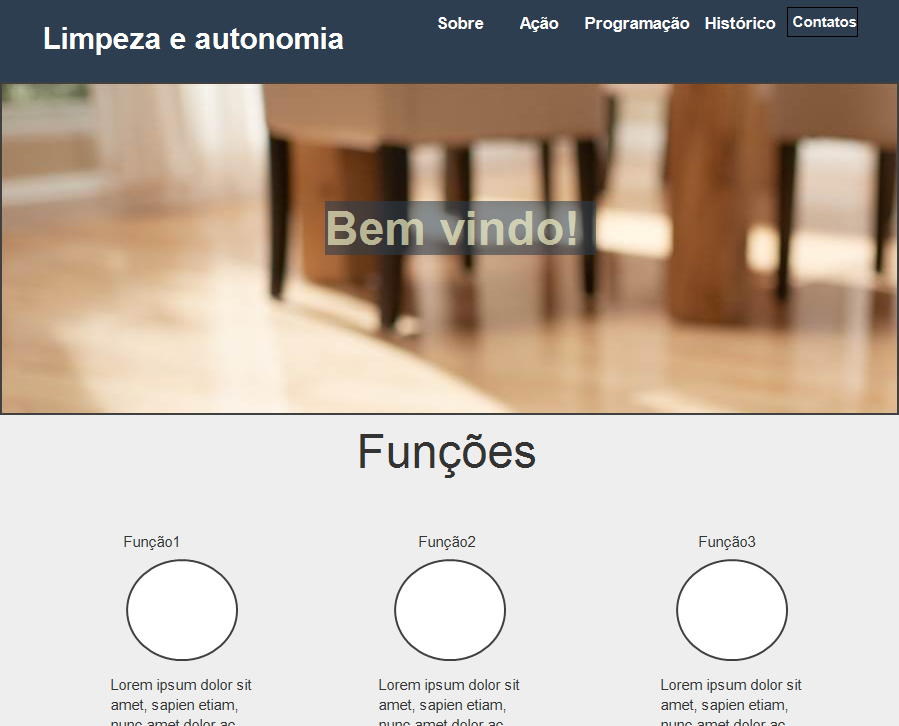
\includegraphics[scale=0.4]{figuras/home.png}
  \caption{Interfaface Home.}                        
  \label{img:inter_home}                              
\end{figure}                                         

\begin{figure}[H]                                    
  \centering                                         
  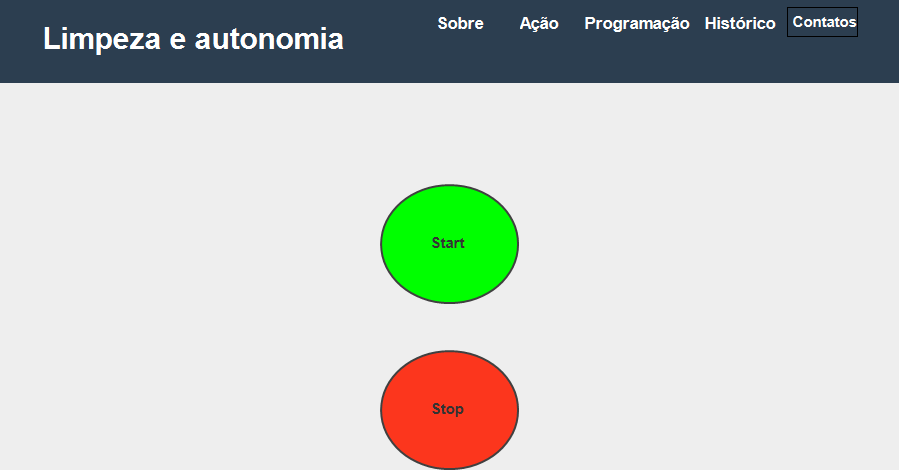
\includegraphics[scale=0.4]{figuras/comando.png}
  \caption{Interfaface Comando.}                        
  \label{img:inter_comando}                              
\end{figure}

\begin{figure}[H]                                    
  \centering                                         
  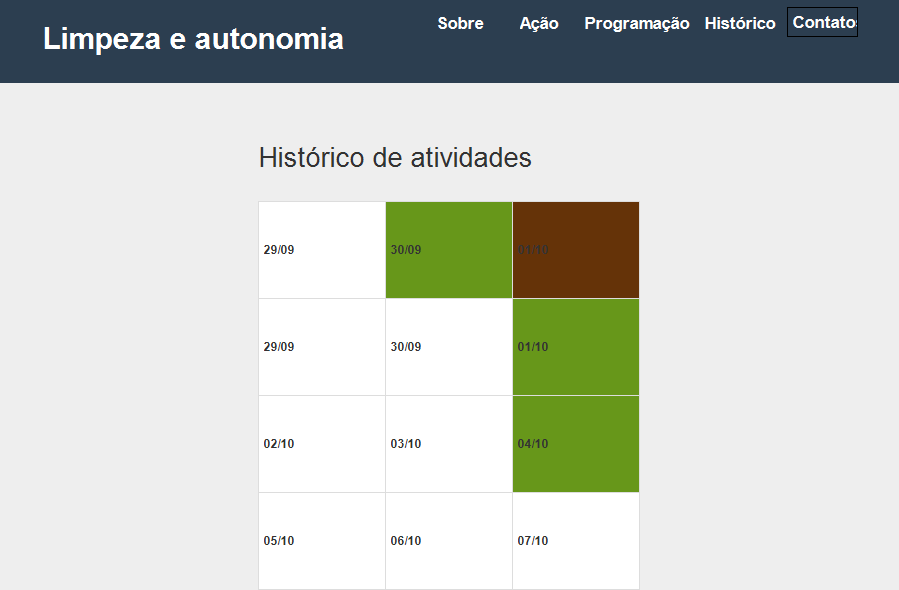
\includegraphics[scale=0.4]{figuras/historico.png}
  \caption{Interfaface Histórico.}                        
  \label{img:inter_historico}                              
\end{figure}

\begin{figure}[H]                                    
  \centering                                         
  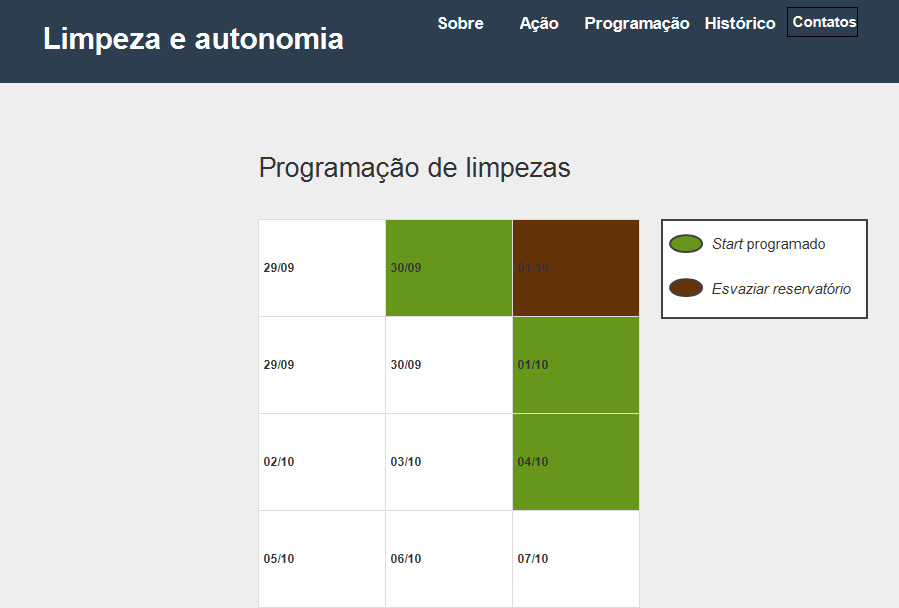
\includegraphics[scale=0.4]{figuras/programacao.png}
  \caption{Interfaface Programação.}                        
  \label{img:inter_programacao}                              
\end{figure}
% section interface (end)
